\maketitle
\tableofcontents
\newpage

\section{Zielsetzung}
Ziel des Versuches ist es, die \textbf{Leerlaufspannung} und den \textbf{\textbf{Innenwiderstand}}
verschiedener Spannungsquellen zu ermitteln.
\section{Theorie}
Die \textbf{Leerlaufspannung} $U_0$ ist die Spannung, die gemessen wird, wenn kein Strom fließt.
Sie wird direkt an den Klemmen der Spannungsquelle abgenommen. Wenn über einen Verbraucher
mit Lastwiderstand $R_a$ ein endlicher Strom $I$ fließt, dann gilt für die nun gemessene
"Klemmenspannung" $U_k$, die ebenfalls an den Klemmen der Spannungsquelle abgenommen wird,
\begin{equation*}
    U_k < U_0 \ .
\end{equation*}
Mit dem zweiten Kirchoffschen Gesetz
\begin{equation}
  \sum_n U_{0_n} = \sum_m R_m \, I_m
  \label{eqn:4}
\end{equation}
folgt für die betrachtete Situation
\begin{equation}
    U_0 = I \, R_i + I \, R_a \ .
    \label{eqn:5}
\end{equation}
\begin{figure}[h]
  \centering
  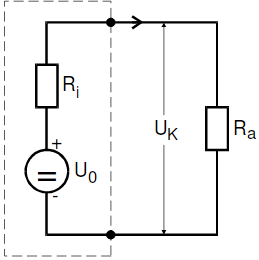
\includegraphics[scale=0.7]{theorie.png}
  \caption{Schaltbild einer idealen Spannungsquelle mit Außenwiderstand $R_i$ und
  Lastwiderstand $R_a$.}
  \label{fig:1}
\end{figure}
Dabei ist $R_i$ der \textbf{\textbf{Innenwiderstand}} der Spannungsquelle. Die Klemmenspannung
$U_k$, siehe \ref{fig:1}, lässt sich somit bestimmen aus \eqref{eqn:5}
\begin{equation}
    U_k = I \, R_a = U_0 - I \, R_i \ .
    \label{eqn:6}
\end{equation}
Damit ist auch die Beziehung
\begin{equation*}
    U_k \approx U_0
\end{equation*}
für die \textbf{Leerlaufspannung} gezeigt, da für diesen Fall in \eqref{eqn:6}
$I$ vernachlässigbar klein wird. Für diese Betrachtungsweise ist die Spannungsquelle
eine sogenannte ideale Spannungsquelle mit einem \textbf{Innenwiderstand} von 0 und einem in
Reihe geschalteten Außenwiderstand $R_i$, der den \textbf{Innenwiderstand} simuliert.

Bei einem RC-Generator wird durch die Änderung des Belastungsstroms das elektrische
Verhalten der Quelle festgelegt. In diesem Fall ist der \textbf{Innenwiderstand} eine differentielle
Größe mit
\begin{equation}
  R_i = \frac{\symup dU_k}{\symup d I} \ .
  \label{eqn:7}
\end{equation}

Für eine Schaltung mit einer Gegenspannung größer als $U_0$\footnote{siehe Kapitel \ref{sec:3.2}} gilt
\begin{equation}
    U_k = U_0 + R_i \, I
    \label{eqn:8}
\end{equation}

\section{Durchführung}
\subsection{Versuchsaufbau}
\begin{figure}
  \centering
  \begin{subfigure}{0.45\textwidth}
    \centering
    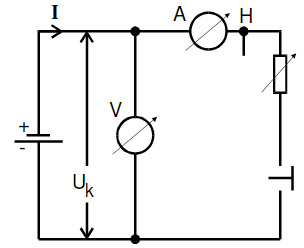
\includegraphics[scale=0.6]{durch.png}
    \caption{Schaltbild zur Messung von $U_k$ in Abhängigkeit von $I$.}
    \label{sub:1}
    \qquad
  \end{subfigure}
  \begin{subfigure}{0.45\textwidth}
    \centering
    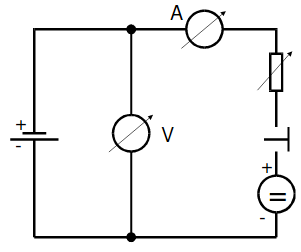
\includegraphics[scale=0.6]{durch2.png}
    \caption{Schaltbild zur Messung von $U_k$ in Abhängigkeit von $I$ mit Gegenspannung.}
    \label{sub:2}
    \qquad
  \end{subfigure}
  \caption{Schaltbilder zu Aufgabe 2 (\ref{sub:1}) und Aufgabe 3 (\ref{sub:2})
  der Versuchsdurchführung.}
  \label{fig:2}
\end{figure}
\subsection{Versuchsdurchführung}
\label{sec:3.2}
Als erstes wurde die \textbf{Leerlaufspannung} einer Monozelle mit einem Spannungsmesser
und der Eingangswiderstand $R_v$ bestimmt. Danach wurde mit der Schaltung in \ref{sub:1}
die Klemmspannung $U_k$ in Abhängigkeit von $I$ gemessen. Der Variationsbereich des
Belastungswiderstandes $R_a$ liegt zwischen 0 und $\SI{50}{\ohm}$ mit einer
Schrittweite von $\SI{5}{\ohm}$.

Als nächstes wurde die Schaltung \ref{sub:2} aufgebaut und die Messung wiederholt.
Dabei ist die Gegenspannung $\SI{2}{\volt}$ größer als die der Monozelle und der
Stromfluss kehrt sich um.

Als letzes wird die Monozelle durch eine Rechteck- und eine Sinusspannung, die
durch einen RC-Generator erzeugt werden, ausgetauscht. Die Variationsbereiche der
Belastungswiderstände lauten:
\begin{itemize}
  \item Sinusspannung: 20 $\leq$ $R_a$ $\le$ $\SI{250}{\ohm}$
  \item Rechteckspannung: 0,1 $\leq$ $R_a$ $\leq$ $\SI{5}{\kilo\ohm}$
\end{itemize}
Die beiden Spannungen haben eine Frequenz von $\SI{50}{\hertz}$, eine Range von $\SI{1}{\volt}$
und wurden mit maximaler Amplitude ausgegeben.
\section{Fehlerrechnung}
Falls zwei fehlerbehaftete Größen in einer Gleichung
 zur Bestimmung einer anderen Größe Verwendung finden, dann berechnte sich der Gesamtfehler
 nach der Gaußschen Fehlerfortpflanzung zu
 \begin{equation}
     \symup \Delta f(x_1, x_2, ..., x_n) = \sqrt{\left(\frac{\symup df}{\symup dx_1} \symup \Delta
     x_1 \right)^2 +    \left(\frac{\symup df}{\symup dx_2} \symup \Delta
     x_2 \right)^2 + ... + \left(\frac{\symup df}{\symup dx_n} \symup \Delta x_n \right)^2} \ .
     \label{eqn:3}
 \end{equation}
\section{Auswertung}
\subsection{Bestimmung von Leerlaufspannung und Innenwiderstand der verschiedenen Spannungsquellen}
\label{sec:5.1}
\begin{figure}[h]
  \begin{subfigure}{0.74\textwidth}
  \centering
    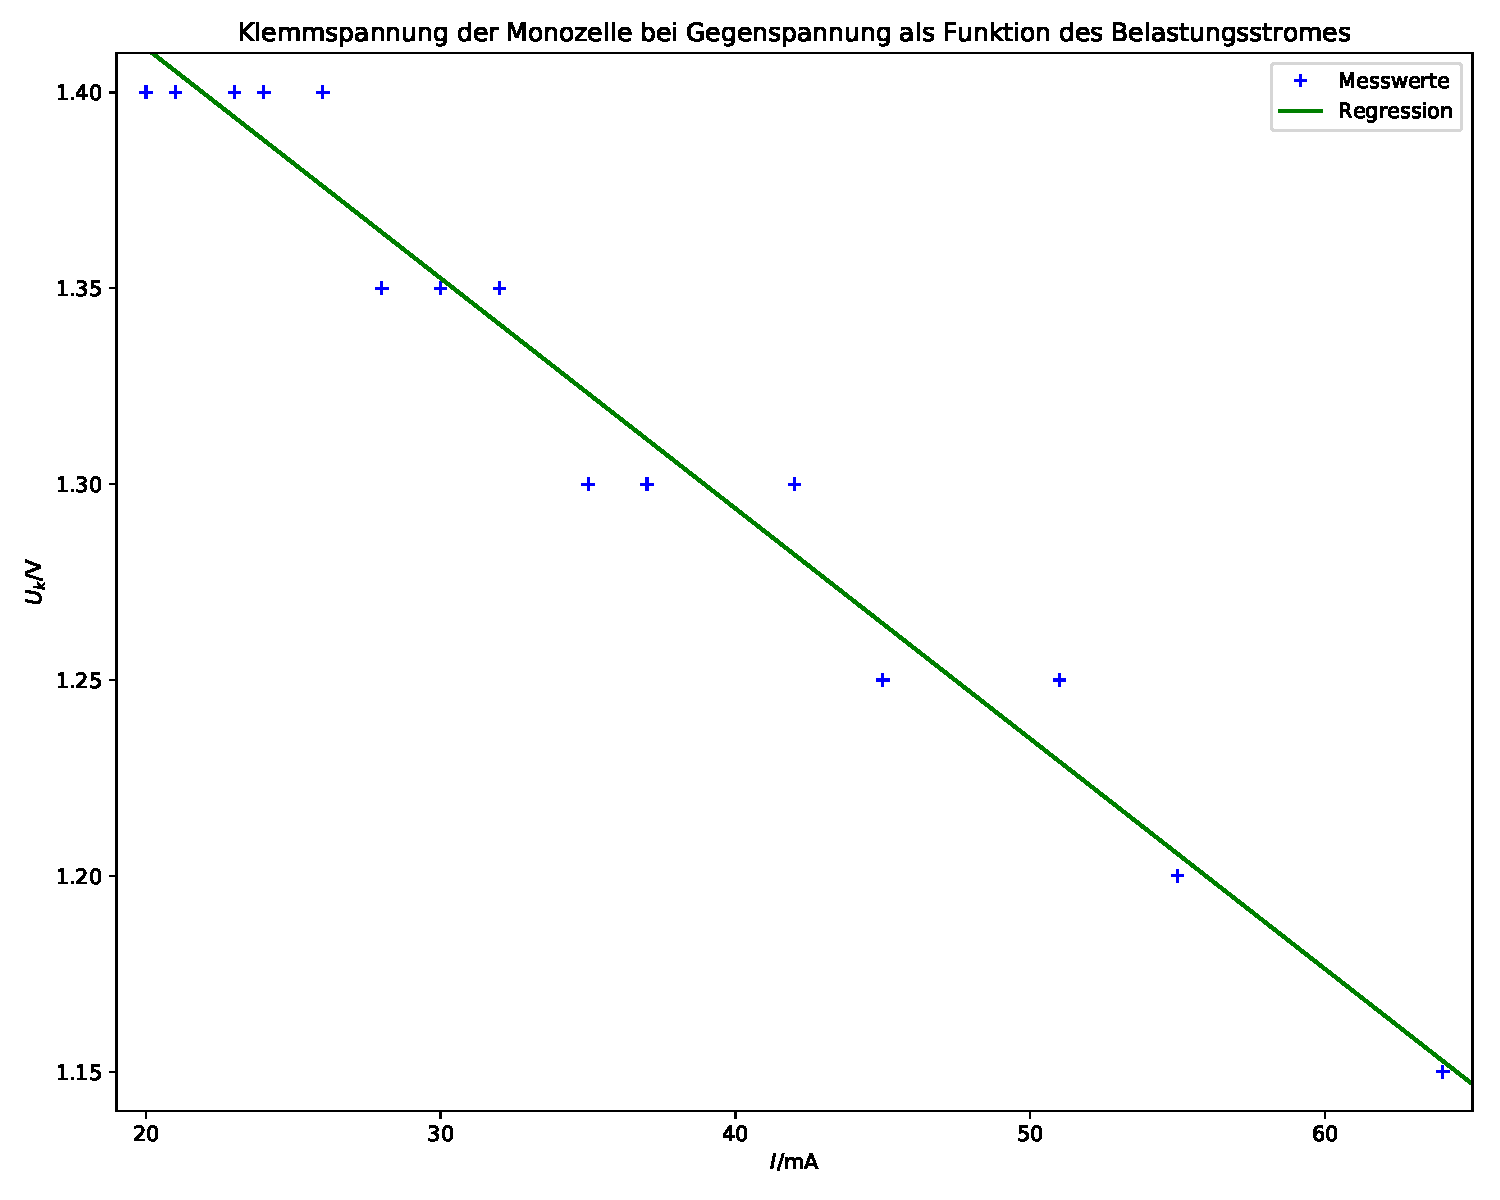
\includegraphics[width=\textwidth]{Mono.pdf}
    \label{sub:1}
    \qquad
  \end{subfigure}
  \begin{subtable}{0.25\textwidth}
  \centering
    \begin{tabular}{c c c}
    \toprule
    $R_a$/$\si{\ohm}$ & $U_{k}/\si{\volt}$ & $I/\si{\milli\ampere}$ \\
    \midrule
    3.46 & 0.45 & 130 \\
    9.38 & 0.75 & 80 \\
    18.00 & 0.90 & 50 \\
    36.67 & 1.10 & 30 \\
    55.00 & 1.10 & 20 \\
    \multicolumn{3} {c}{hier Skalenwechsel}\\
    17.97 & 1.15 & 64 \\
    21.82 & 1.20 & 55 \\
    24.51 & 1.25 & 51 \\
    27.78 & 1.25 & 45 \\
    30.95 & 1.30 & 42 \\
    35.14 & 1.30 & 37 \\
    37.14 & 1.30 & 35 \\
    42.19 & 1.35 & 32 \\
    45.00 & 1.35 & 30 \\
    48.21 & 1.35 & 28 \\
    53.85 & 1.40 & 26 \\
    58.33 & 1.40 & 24 \\
    60.87 & 1.40 & 23 \\
    66.67 & 1.40 & 21 \\
    70.00 & 1.40 & 20 \\
    \bottomrule
    \end{tabular}
    \label{sub:2}
    \qquad
  \end{subtable}
  \caption{In der Grafik wurden die Klemmspannungen an der Monozelle gegen die gemessenen Stromstärken aufgetragen. Die Werte vor
  Umstellung der Skala des Amperemeters wurden in der Grafik vernachlässigt. Die Tabelle zeigt die Messwerte und die
   nach $R = U/I$ bestimmten Widerstände}
  \label{tabplot:1}
\end{figure}

Grafik und Messwerte für die Messung an der Monozelle finden sich in Grafik \ref{tabplot:1}. Nach einer
Umstellung der Skala des Spannungsmessgerätes, die während der Messung notwendig wurde, ergaben sich
mit den vorherigen Werten inkonsistente Ergebnisse. Daher werden die 5 vor der Umstellung genommenen Messwerte
in der Grafik nicht betrachtet.\\
\\
Aufgrund des Zusammenhanges in \eqref{eqn:6} lassen sich $U_0$ und $R_i$ durch lineare Regression berrechnen.
Die Regression ist in Grafik \ref{tabplot:1} dargestellt. Es ergeben sich:
\begin{equation*}
  \begin{split}
    U_0 = \SI{1.529(11)}{\volt}\\
    R_I = \SI{5.87(30)}{\ohm}
  \end{split}
\end{equation*}
\newpage
\begin{figure}[h]
  \begin{subfigure}{0.74\textwidth}
  \centering
    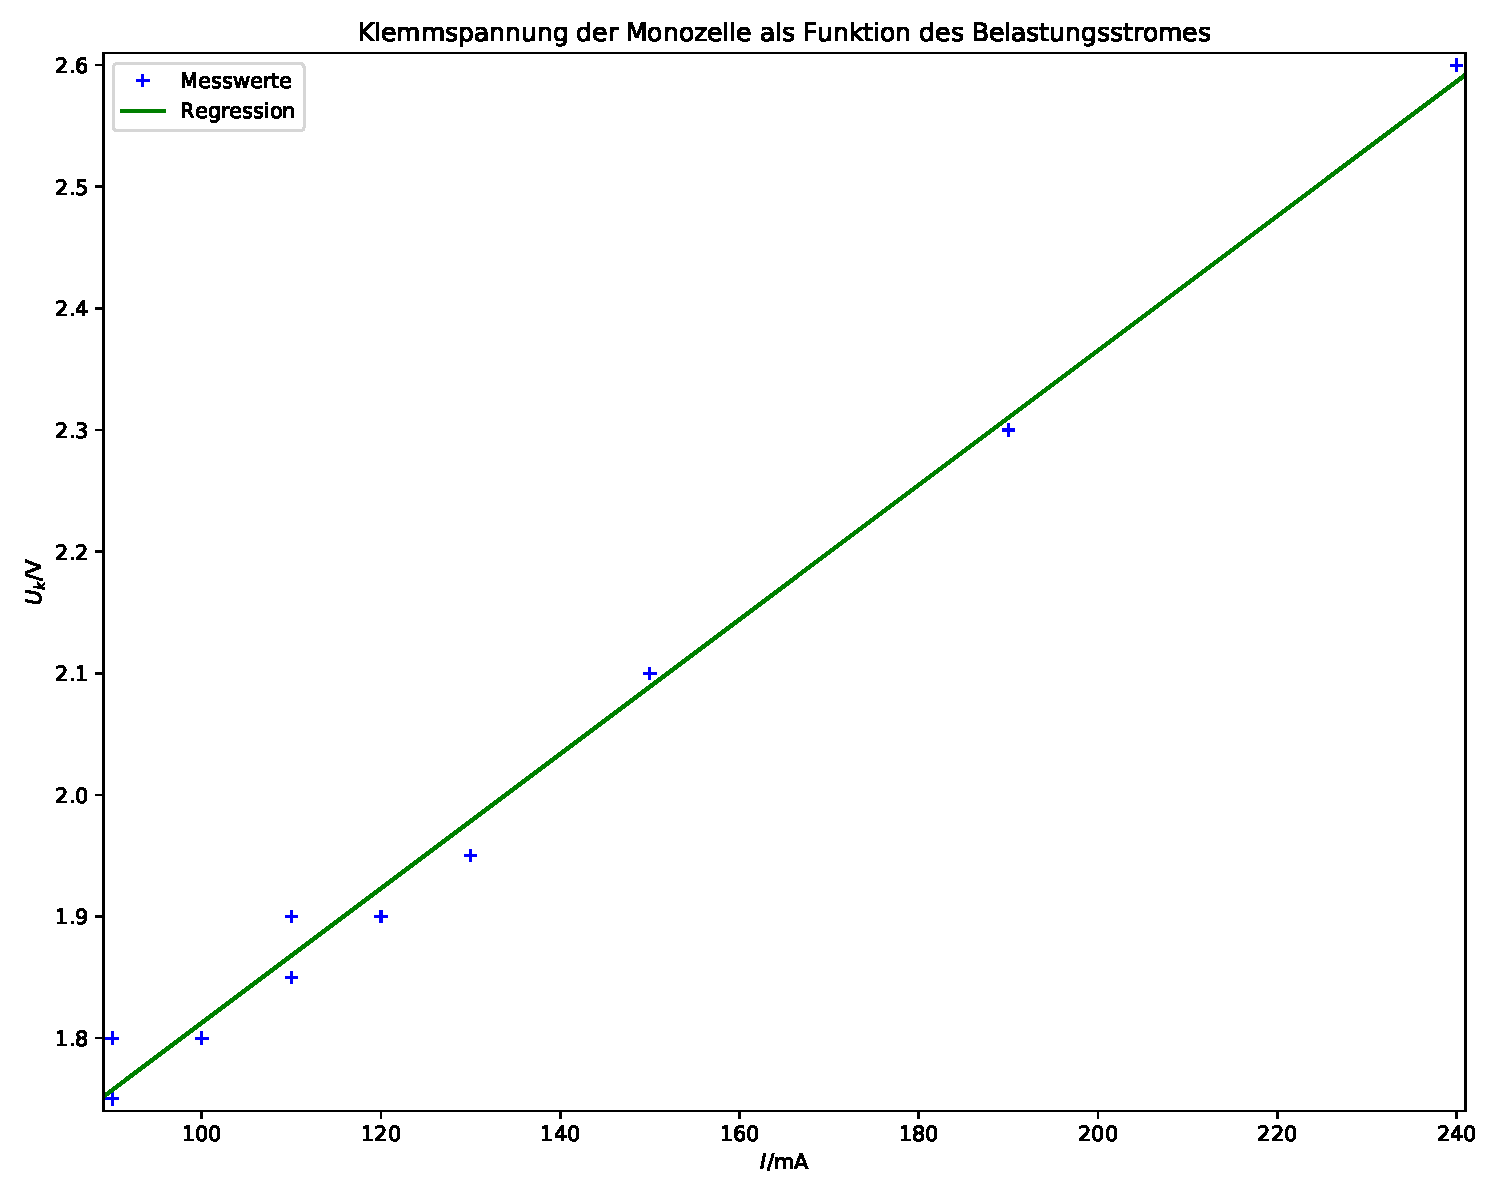
\includegraphics[width=\textwidth]{MonoGegen.pdf}
    \label{sub:3}
    \qquad
  \end{subfigure}
  \begin{subtable}{0.25\textwidth}
  \centering
    \begin{tabular}{c c c}
    \toprule
    $R_a$/$\si{\ohm}$ & $U_{k}/\si{\volt}$ & $I/\si{\milli\ampere}$ \\
    \midrule
    10.83 & 2.60 & 240 \\
    12.11 & 2.30 & 190 \\
    14.00 & 2.10 & 150 \\
    15.00 & 1.95 & 130 \\
    15.83 & 1.90 & 120 \\
    17.27 & 1.90 & 110 \\
    16.82 & 1.85 & 110 \\
    18.00 & 1.80 & 100 \\
    20.00 & 1.80 & 90 \\
    19.44 & 1.75 & 90 \\
    \bottomrule
    \end{tabular}
    \label{sub:4}
    \qquad
  \end{subtable}
  \caption{In der Grafik wurden die Klemmspannungen an der Monozelle bei Gegenspannung
  gegen die gemessenen Stromstärken aufgetragen. Die Tabelle zeigt die Messwerte und die
   nach $R = U/I$ bestimmten Widerstände}
  \label{tabplot:2}
\end{figure}

In Grafik \ref{tabplot:2} sind Messwerte und Grafik mit Regression an der Monozelle bei Gegenspannung
dargestellt. Aus der Regression folgt wie oben:
\begin{equation*}
  \begin{split}
    U_0 = \SI{1.260(25)}{\volt}\\
    R_I = \SI{5.53(17)}{\ohm}
  \end{split}
\end{equation*}
Im Vergleich mit der Messung ohne Gegenspannung zeigt sich, dass die Abweichung der Werte für den Innenwiderstand
im Bereich der Messungenauigkeit liegen.
\begin{figure}[h]
  \begin{subfigure}{0.74\textwidth}
  \centering
    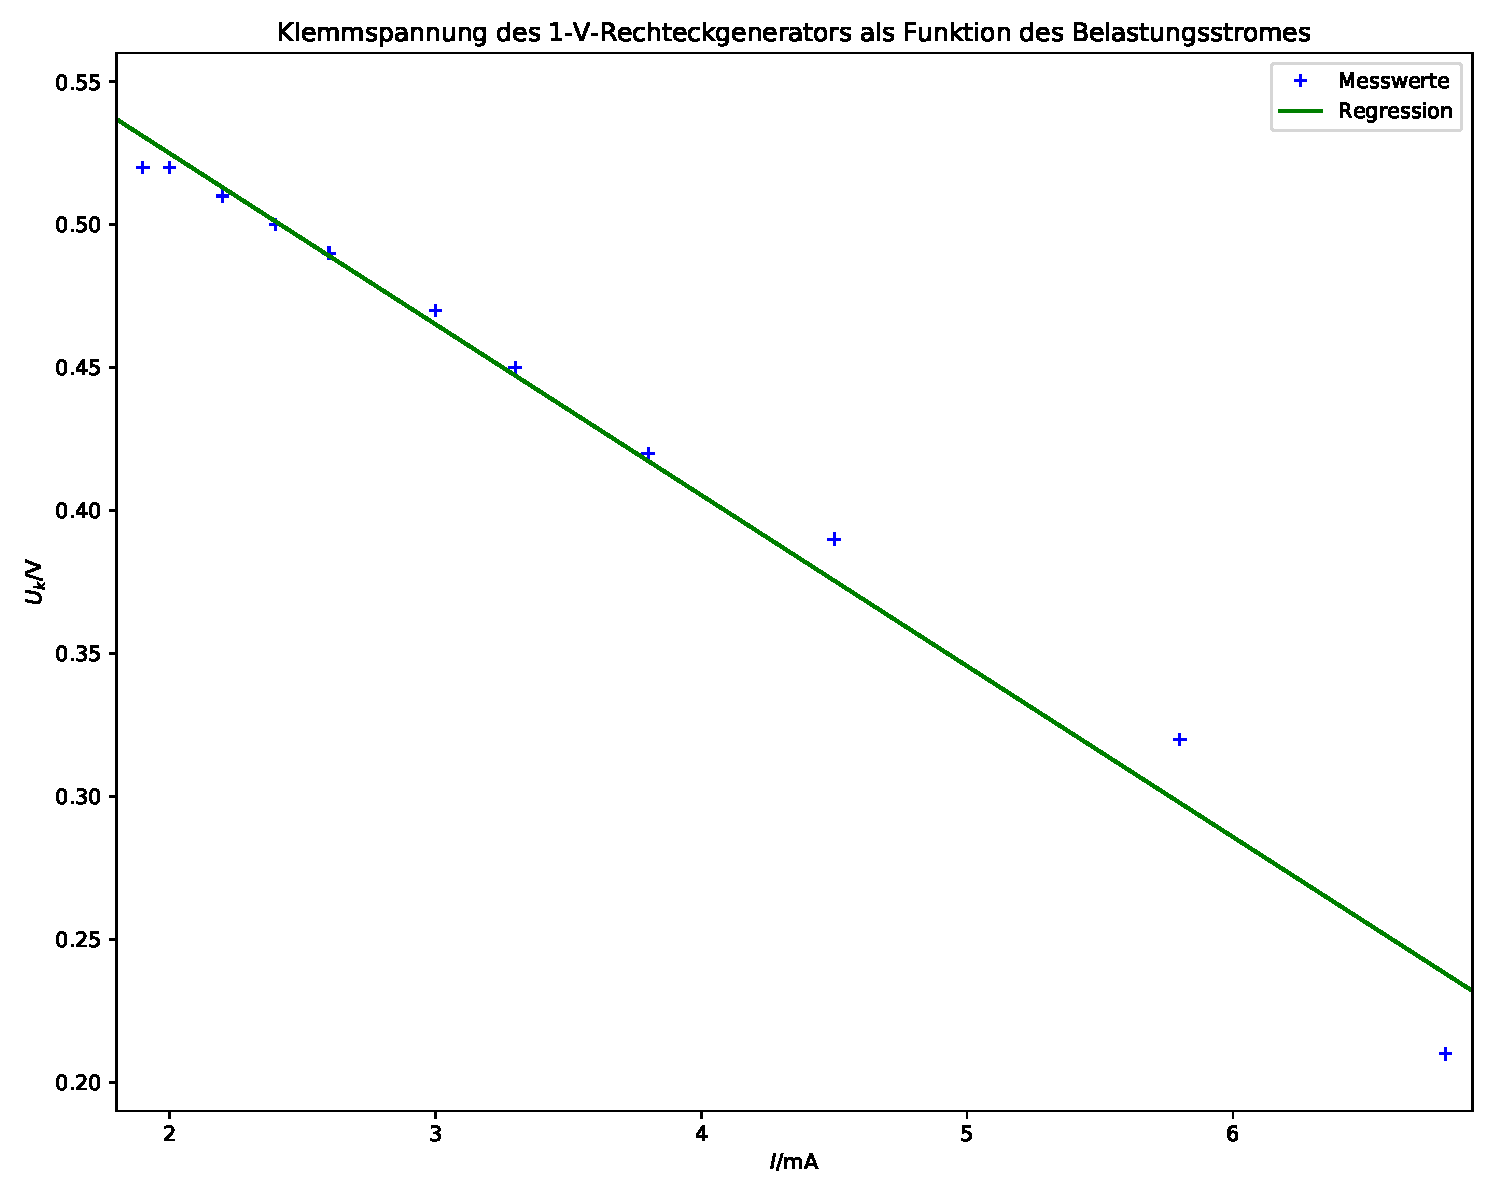
\includegraphics[width=\textwidth]{Rechteck.pdf}
    \label{sub:5}
    \qquad
  \end{subfigure}
  \begin{subtable}{0.25\textwidth}
  \centering
    \begin{tabular}{c c c}
    \toprule
    $R_a$/$\si{\ohm}$ & $U_{k}/\si{\volt}$ & $I/\si{\milli\ampere}$ \\
    \midrule
    273.68 & 0.52 & 1.9 \\
    260.00 & 0.52 & 2.0 \\
    231.82 & 0.51 & 2.2 \\
    208.33 & 0.50 & 2.4 \\
    188.46 & 0.49 & 2.6 \\
    156.67 & 0.47 & 3.0 \\
    136.36 & 0.45 & 3.3 \\
    110.53 & 0.42 & 3.8 \\
    86.67 & 0.39 & 4.5 \\
    55.17 & 0.32 & 5.8 \\
    30.88 & 0.21 & 6.8 \\
    \bottomrule
    \end{tabular}
    \label{sub:6}
    \qquad
  \end{subtable}
  \caption{In der Grafik wurden die Klemmspannungen am Rechteckausgang eines RC-Generators
  gegen die gemessenen Stromstärken aufgetragen. Die Tabelle zeigt die Messwerte und die
   nach $R = U/I$ bestimmten Widerstände}
  \label{tabplot:3}
\end{figure}

\begin{figure}[h]
  \begin{subfigure}{0.74\textwidth}
  \centering
    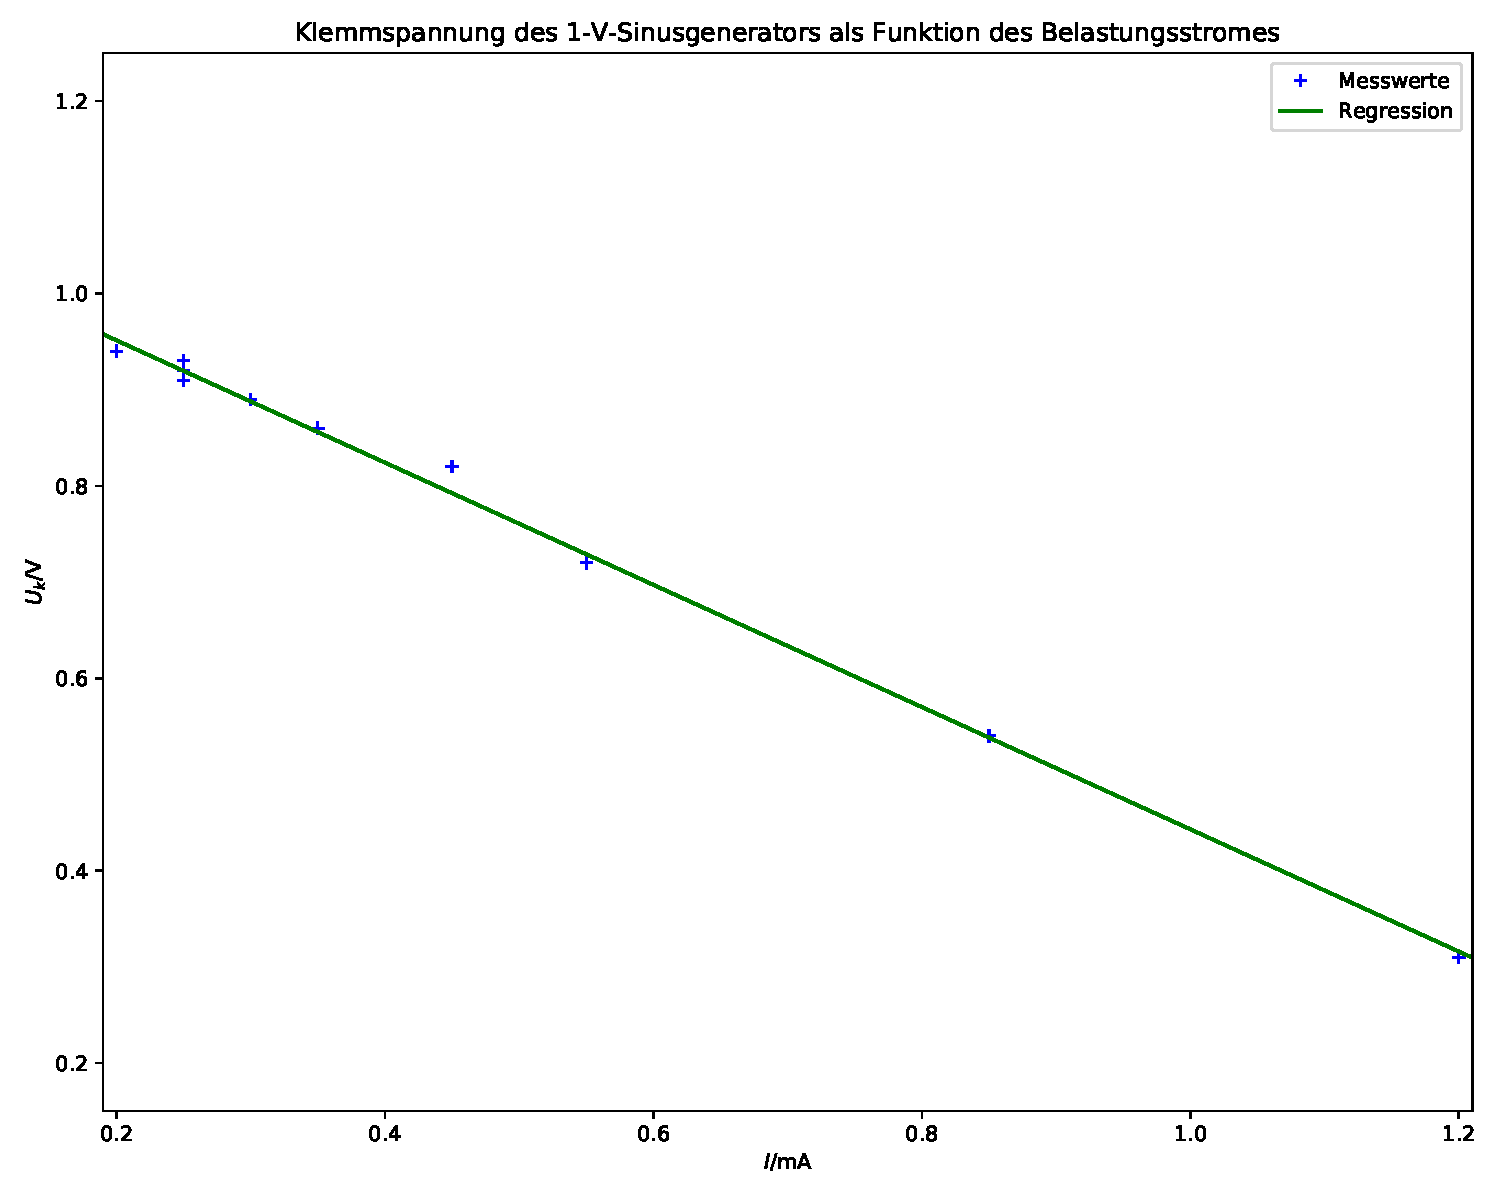
\includegraphics[width=\textwidth]{Sinus.pdf}
    \label{sub:7}
    \qquad
  \end{subfigure}
  \begin{subtable}{0.25\textwidth}
  \centering
    \begin{tabular}{c c c}
    \toprule
    $R_a$/$\si{\kilo\ohm}$ & $U_{k}/\si{\volt}$ & $I/\si{\milli\ampere}$ \\
    \midrule
    4.70 & 0.94 & 0.20 \\
    4.70 & 0.94 & 0.20 \\
    3.72 & 0.93 & 0.25 \\
    3.68 & 0.92 & 0.25 \\
    3.64 & 0.91 & 0.25 \\
    2.97 & 0.89 & 0.30 \\
    2.46 & 0.86 & 0.35 \\
    1.82 & 0.82 & 0.45 \\
    1.31 & 0.72 & 0.55 \\
    0.64 & 0.54 & 0.85 \\
    0.26 & 0.31 & 1.20 \\
    \bottomrule
    \end{tabular}
    \label{sub:8}
    \qquad
  \end{subtable}
  \caption{In der Grafik wurden die Klemmspannungen am Sinusausgang eines RC-Generators
  gegen die gemessenen Stromstärken aufgetragen. Die Tabelle zeigt die Messwerte und die
   nach $R = U/I$ bestimmten Widerstände}
  \label{tabplot:4}
\end{figure}
Grafik mit Regression und die jeweiligen Messwerte finden sich in Grafik \ref{tabplot:3} für den
Rechteckausgang und in \ref{tabplot:4} für den Sinusausgang. Aus der Regression folgt wieder für
den Rechteckausgang:
\begin{equation*}
  \begin{split}
    U_0 = \SI{0.644(10)}{\volt}\\
    R_I = \SI{59.8(27)}{\ohm}
  \end{split}
\end{equation*}
und für den Sinusausgang:
\begin{equation*}
  \begin{split}
    U_0 = \SI{1.078(7)}{\volt}\\
    R_I = \SI{635(12)}{\ohm}
  \end{split}
\end{equation*}
\newpage
\subsection{Direkte Messung der Leerlaufspannung}
Für den durch den endlichen Eingangswiderstand $R_v$ des Voltmeters von $\geq \SI{10}{\mega\ohm}$ entstehenden,
systematischen Fehler bei der Spannungsmessung, folgt aus \eqref{eqn:6} unter Verwendung von \eqref{eqn:3}:
\begin{equation}
  U_0 - U_k = U_k \, \frac{R_i}{R_v} = \symup{\Delta} \, U
  \label{eqn:9}
\end{equation}
Daraus ergibt sich für die Monozelle, bei einer gemessenenen Spannung
\begin{equation*}
  \begin{split}
    U_k = \SI{1.55}{\volt}
  \end{split}
\end{equation*}
und dem in Kapitel \ref{sec:5.1} berechneten Innenwiderstand der Spannungsquelle $R_i$
für $\symup{\Delta} \, U$:
\begin{equation*}
  \symup{\Delta} \, U = \SI{9.1(5)e-07}{\volt}
\end{equation*}
Dieser Wert ist so gering, dass er vernachlässigt werden kann. Die direkte Messung der
Leerlaufspannung kann somit als genau angenommen werden. Im Vergleich mit der in \ref{sec:5.1}
berechneten Leerlaufspannung zeigt sich, dass diese leicht unter der hier bestimmten liegt.
Die Abweichung liegt dennoch nicht im Bereich der Messungenauigkeit.\\
\\
Eine im Gegensatz zum Voltmeter messbare systematische Fehlerquelle wäre das Legen
des Voltmeters hinter das Amperemeter. Am realen Widerstand des Amperemeters fällt ein Teil
der Spannung ab, sodass eine Messung nach dem Amperemeter nicht die Klemmspannung an der Monozelle
messen kann.
\subsection{Leistungsabfall am Belastungswiderstand}
Wird die Leistung betrachtet, die am Belastungswiderstand umgesetzt wird, so folgt aus \eqref{eqn:3}
mit $N = U_k \, I$:
\begin{equation}
  N(R_a) = \frac{{U_0}^2 \, R_a}{(R_a + R_i)^2}
  \label{eqn:10}
\end{equation}
Wird nun $N = U_k \, I$ gegen $R_a = U_k/I$ aufgetragen und zusätzlich $N(R_a)$ in die Grafik
eingetragen, so ergibt sich der in Grafik \ref{tabplot:5} dargestellte Verlauf. Die Fehler folgen nach
\eqref{eqn:3} aus der Fehlerbehafteten Größe $R_i$. Es zeigt sich eine gute Übereinstimmung zwischen der
Kurve und den Berechneten Werten für $N$.

\begin{figure}[h]
  \begin{subfigure}{0.74\textwidth}
  \centering
    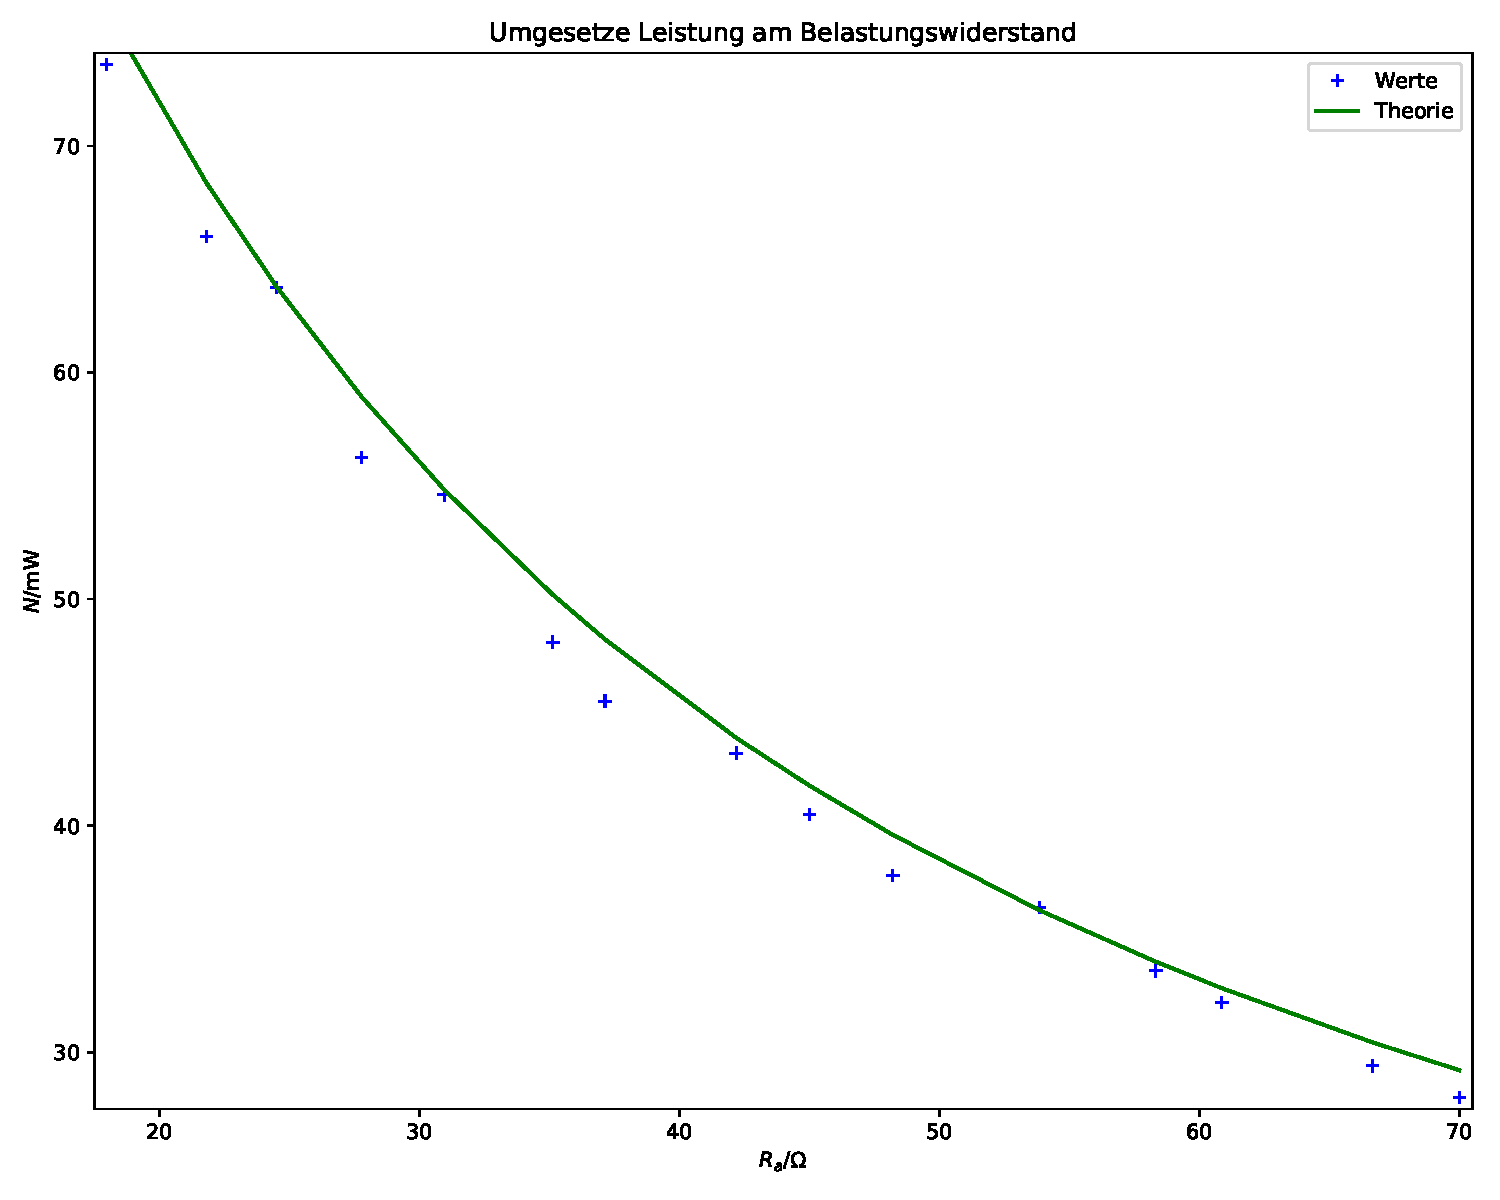
\includegraphics[width=\textwidth]{Leistung.pdf}
    \label{sub:9}
    \qquad
  \end{subfigure}
  \begin{subtable}{0.25\textwidth}
  \centering
    \begin{tabular}{c c c}
    \toprule
    $R_a$/$\si{\ohm}$ & $N/\si{\milli\watt}$ & $N(R_a)/\si{\milli\watt}$ \\
    \midrule
    17.97 & 73.60 & \num{75,94(190)} \\
    21.82 & 66.00 & \num{68,35(147)} \\
    24.51 & 63.75 & \num{63,78(125)} \\
    27.78 & 56.25 & \num{58,93(105)} \\
    30.95 & 54.60 & \num{54,83(89)} \\
    35.14 & 48.10 & \num{50,19(73)} \\
    37.14 & 45.50 & \num{48,22(66)} \\
    42.19 & 43.20 & \num{43,88(55)} \\
    45.00 & 40.50 & \num{41,77(49)} \\
    48.21 & 37.80 & \num{39,59(44)} \\
    53.85 & 36.40 & \num{36,27(36)} \\
    58.33 & 33.60 & \num{33,99(32)} \\
    60.87 & 32.20 & \num{32,83(29)} \\
    66.67 & 29.40 & \num{30,44(25)} \\
    70.00 & 28.00 & \num{29,21(23)} \\
    \bottomrule
    \end{tabular}
    \label{sub:10}
    \qquad
  \end{subtable}
  \caption{In der Grafik wurde der Leistungsumsatz am Belastungswiderstand bei Messung der Monozelle
  dargestellt. Die Tabelle enthält die dazugehörigen Messwerte.}
  \label{tabplot:5}
\end{figure}

\section{Diskussion}
Zusammenfassend zeigen sich besonders bei der Monozelle zwischen den drei Messmethoden
untereinander schlüssige Werte, die sich teilweise (Monozelle mit und ohne Gegenspannung)
im Bereich der Messungenauigkeit befinden, beziehungsweise nur leicht unterscheiden (Monozelle bei Variation des Belastungswiderstandes
und direkte Messung). Bei den Ausgängen am RC-Generator fehlt eine Vergleichsmöglichkeit.

Problematisch waren die ungenauen Multimeter, die eine Änderung in Größenordnungen unterhalb
der Skala kaum anzeigen können (Siehe Grafik \ref{tabplot:1}, man erkennt, dass kleine Änderungen
der Werte nicht abgelesen werden konnten, was zu einer scheinbar diskreten Verteilung der Messwerte führt).
Ein Verstellen der Skala war gleichzeitig jedoch nicht möglich, da sich dabei,
wie in Kapitel \ref{sec:5.1} ersichtlich, die Ergebnisse verfälschen. Es empfiehlt sich daher
eine Wiederholung des Experimentes mit einem digitalen Messgerät, oder einem analogen Gerät mit
größerer Skalenweite, um die Werte zu überprüfen. Auch eine Messung nach einer anderen Methode, wie
zum Beispiel der "Nullmethode" würde zum Verifizieren der Daten beitragen.

Als systematischer Fehler quasi ausschließen lässt sich der endliche Innenwiderstand des Voltmeters.
Der dadurch entstandene Fehler liegt in einer Größenordnung, in der keine Messungen mehr möglich
waren. Der Fehler kann daher nicht in die Messwerte einfließen.
\newpage
\nocite{*}
\printbibliography
